\chapter{基于$C_4$对称的声学拓扑晶体绝缘体的声传播与彩虹捕获研究}
\section{引言}
在上一章节中,我们讨论了亚波长尺度下,腔管结构的声学拓扑绝缘体的构造方法,并观察了其高阶拓扑态。一方面,对于如上一章节提到的无自旋并且时间反演不变的拓扑晶体绝缘体而言,其独特的拓扑态是由体极化来进行表征的。这种特性使得拓扑边界态在界面处有很强的鲁棒性。另一方面,我们的声学建模为在声学系统中实现这一类拓扑绝缘体提供了理论基础,我们可以根据理论模型里的相互作用,设计出对应尺寸的声学结构。如此一来,声学拓扑晶体绝缘体便自然而然地为利用特定的能量(也就是特定的频率)在结构的边界或者角落之处,以一种鲁棒的方式俘获波提供了一个极为理想的平台。

然而,尽管已经有大量细致入微的研究,无论是从理论层面还是实验层面,都确凿地证明了拓扑晶体绝缘体(TCIs)中存在着拓扑态,但是,像拓扑态的群速度这类与传播特性相关的内容,却鲜少被人们深入地探讨和研究。可实际上,这些传播特性在拓扑晶体绝缘体的实际应用当中,却是一个至关重要且无法回避的问题。

举个例子来说,利用拓扑态来实现彩虹俘获就是一个典型的应用场景。所谓的彩虹俘获,指的是将具有不同频率的波进行分离,并且让它们分别被俘获在不同的空间位置上。这种现象已经在多个领域的系统中被提出,比如在电磁波系统\cite{C41-1,C41-2,C41-3,C41-4,C41-5,C41-6,C41-7,C41-8,C41-9}、弹性波系统\cite{C42-1,C42-2,C42-3,C42-4,C42-5,C42-6}以及空气声系统\cite{C43-1,C43-2,C43-3,C43-4}中。在这些相关的研究工作里,研究人员们纷纷采用了各种各样的方法,其目的就是为了能够控制不同系统中波的色散关系,从而使得波能够在空间的不同位置上实现局域化。

不仅如此,一些近期的研究工作更是已经在拓扑态中成功地实现了彩虹俘获\cite{C44-1,C44-2,C44-3,C44-4,C44-5,C44-6}。在这些研究中,隙内模式能够在不减小体带隙的情况下被有效地减慢,而且体带隙依然能够受到强无序的良好保护。不过,令人遗憾的是,现有的这些方法通常都需要在体中设置额外的区域或者对晶格进行相应的变化。例如,在左边非平庸介质A和右边平庸的介质B构造一个界面,而拓扑边界态出现在中间的A和B界面之间,亦或是在平庸的环境中嵌入非平庸的介质,使得拓扑边界态出现在嵌入的非平庸介质周界。然而,在上一章节里,我们揭示了仅需要调控非平庸的声学结构以及边界条件,即可实现拓扑边界态。进一步,从实际应用的角度出发,我们还需要一种全新的方法,这种方法能够直接对边界处拓扑态的传播速度进行有效的控制。

因此,本章工作的目的是提出一种控制拓扑晶体绝缘体中不同频率下声波传播速度的方法,以实现声学彩虹俘获。基于二维(2D)Su-Schrieffer-Heeger(SSH)模型,我们严格证明了经典波系统的阻抗与紧束缚模型的跳跃项和在位项之间的对应关系,这表明,无需对体进行变形,通过仅仅调节超材料的表面阻抗,就可以精确且独立地控制边界态的群速度。这一特性天然为拓扑保护波俘获提供了一个新的思路,使得我们能利用边界态的鲁棒性的同时,也能大大减小结构的尺寸。由此我们通过实验展示了一个亚波长拓扑彩虹集中器的原型,其理论、仿真和实验结果显示这一结构可以时不同频率的声波停驻在拓扑绝缘体边界的不同位置。

本章主要内容如下:4.2节基于二维 SSH 声学拓扑晶体绝缘体,研究了体系的拓扑性质并深入探讨该绝缘体的特性以及在位势对其产生的影响等相关内容。4.3节着重阐述改变拓扑边界态的传播情况的相关原理,提出了改变表面阻抗从而改变拓扑边界态的群速度的方法。4.4节则围绕拓扑彩虹俘获的实验展开,详细介绍实现这一现象的具体过程、技术和相关要点。最后,4.5 节进行小结。

\section{二维SSH理论模型的能带结构和拓扑不变量}

\begin{figure}[h!]
    \centering
    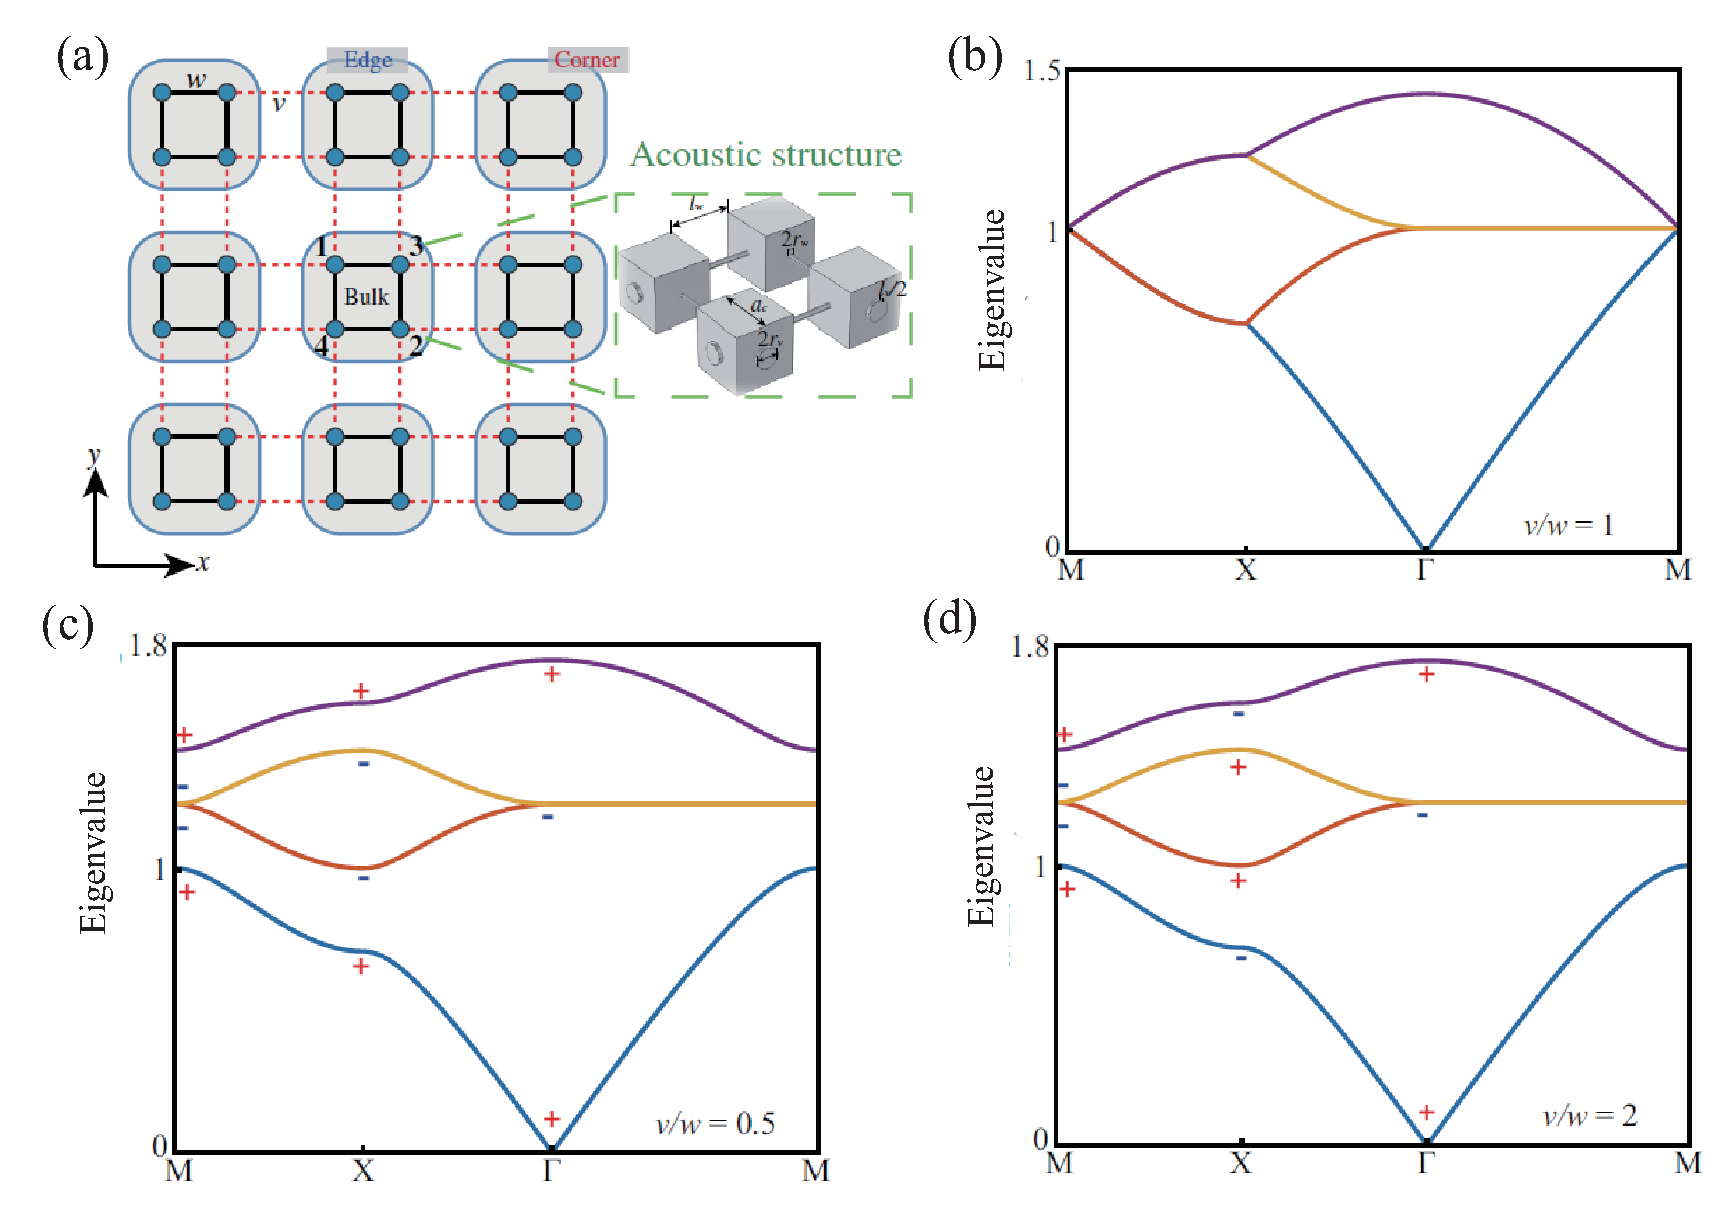
\includegraphics[width=1\textwidth]{images/fig4-1.eps} 
    \caption{(a) 二维SSH模型的示意图。(b-d)二维SSH模型的理论体能量带结构:(b)$v/w = 1$、(c)$v/w = 0.5$和(c)$v/w = 2$,“+/−”符号表示在高对称点处态的偶(+)奇(−)宇称。}
    \label{fig_4_1}
  \end{figure}  

在这部分,我们展示二维SSH紧束缚模型与声波系统之间对应关系的推导,并介绍其能带结构。首先,我们专注于线性经典波系统,并从如图\ref{fig_4_1}(a)所示的典型二维SSH模型开始,其中插图展示了相应的声学结构。用上一章节介绍的电子系统和声学系统类比思路,该结构用腔体模拟原子,用管道模拟格点跳跃。其中,正方体腔体的边长位$a_c$,胞内和胞间导管的长度分别为$l_w$和$l_v$,半径分别为$r_w$和$r_v$。

在这里,我们定义在$(i,j)$晶格处的波函数(在声学系统里,可用声压作波函数)为$\Psi_{i,j} = [\psi_{i,j}^{(1)}, \psi_{i,j}^{(2)}, \psi_{i,j}^{(3)}, \psi_{i,j}^{(4)}]^T$,其中上标表示如文中图\ref{fig_4_1}(a)所标记的原子。通过上一章节展示的等效电路方法和基尔霍夫电流定律,可以得到方程
\begin{equation}
    \begin{aligned}
    -\frac{\psi_{(i,j)}^{(1)}}{Z_c} &= \frac{\psi_{(i,j)}^{(1)} - \psi_{(i,j)}^{(3)}}{Z_w} + \frac{\psi_{(i,j)}^{(1)} - \psi_{(i,j + 1)}^{(4)}}{Z_v} + \frac{\psi_{(i,j)}^{(1)} - \psi_{(i - 1,j)}^{(3)}}{Z_v} + \frac{\psi_{(i,j)}^{(1)} - \psi_{(i,j)}^{(4)}}{Z_w} \\
    -\frac{\psi_{(i,j)}^{(2)}}{Z_c} &= \frac{\psi_{(i,j)}^{(2)} - \psi_{(i,j + 1)}^{(4)}}{Z_v} + \frac{\psi_{(i,j)}^{(2)} - \psi_{(i + 1,j)}^{(3)}}{Z_w} + \frac{\psi_{(i,j)}^{(2)} - \psi_{(i,j)}^{(4)}}{Z_w} + \frac{\psi_{(i,j)}^{(2)} - \psi_{(i,j - 1)}^{(3)}}{Z_v} \\
    -\frac{\psi_{(i,j)}^{(3)}}{Z_c} &= \frac{\psi_{(i,j)}^{(3)} - \psi_{(i + 1,j)}^{(4)}}{Z_v} + \frac{\psi_{(i,j)}^{(3)} - \psi_{(i,j + 1)}^{(1)}}{Z_v} + \frac{\psi_{(i,j)}^{(3)} - \psi_{(i,j)}^{(1)}}{Z_w} + \frac{\psi_{(i,j)}^{(3)} - \psi_{(i,j)}^{(2)}}{Z_w} \\
    -\frac{\psi_{(i,j)}^{(4)}}{Z_c} &= \frac{\psi_{(i,j)}^{(4)} - \psi_{(i,j)}^{(2)}}{Z_w} + \frac{\psi_{(i,j)}^{(4)} - \psi_{(i,j)}^{(1)}}{Z_w} + \frac{\psi_{(i,j)}^{(4)} - \psi_{(i - 1,j)}^{(2)}}{Z_v} + \frac{\psi_{(i,j)}^{(4)} - \psi_{(i,j - 1)}^{(1)}}{Z_v}
    \end{aligned}
    \label{eq4-1}
\end{equation}

由于$Z_w = i\omega L_w$,$Z_v = i\omega L_v$且$Z_c = 1/i\omega C$,我们可以分别定义$w = -1/(L_wC)$和$v = -1/(L_vC)$。然后我们将所考虑的晶格标记为0,其左、下、右和上的最近邻晶格分别标记为$i = 1,2,3,4$。相应地,方程\ref{eq4-1}可重写为
\begin{equation}\label{eq4-2}
    \omega^2\Psi_0 = \hat{H}_0\Psi_0 + \sum_{i = 1}^{4} \hat{H}_i\Psi_i, 
\end{equation}
其中
\begin{equation}\label{eq4-3}
    \hat{H}_0 = 
    \begin{pmatrix}
    -2w - 2v & 0 & w & w \\
    0 & -2w - 2v & w & w \\
    w & w & -2w - 2v & 0 \\
    w & w & 0 & -2w - 2v
    \end{pmatrix}, 
\end{equation}
\begin{equation}\label{eq4-4}
    \hat{H}_1 = 
    \begin{pmatrix}
    0 & 0 & v & 0 \\
    0 & 0 & 0 & 0 \\
    0 & 0 & 0 & 0 \\
    0 & v & 0 & 0
    \end{pmatrix},
    \hat{H}_2 = 
    \begin{pmatrix}
    0 & 0 & 0 & 0 \\
    0 & 0 & v & 0 \\
    0 & 0 & 0 & 0 \\
    v & 0 & 0 & 0
    \end{pmatrix},
    \hat{H}_3 = 
    \begin{pmatrix}
    0 & 0 & 0 & 0 \\
    0 & 0 & 0 & 0 \\
    0 & 0 & 0 & v \\
    0 & 0 & 0 & 0
    \end{pmatrix},
    \hat{H}_4 = 
    \begin{pmatrix}
    0 & 0 & 0 & v \\
    0 & 0 & 0 & 0 \\
    0 & 0 & 0 & 0 \\
    0 & 0 & 0 & 0
    \end{pmatrix}, 
\end{equation}
进一步,通过应用傅里叶展开为
\begin{equation}\label{eq4-5}
    \Psi_0 = \sum_{k} \psi_k e^{i\vec{k} \cdot \vec{r}_0}
\end{equation}
\begin{equation}\label{eq4-6}
    \Psi_i = e^{i\vec{k} \cdot \vec{r}_i} \sum_{k} \psi_k e^{i\vec{k} \cdot \vec{r}_0},
\end{equation}
其中$i = 1,2,3,4$表示晶格0的左、下、右和上的最近邻晶格,$\vec{r}_i$是从晶格0指向它们的位置矢量。方程最终可以写成如下的形式
\begin{equation}\label{eq4-7}
    \omega_k^2 \psi_k = \hat{H}_k \psi_k,
\end{equation}
其中紧束缚模型的哈密顿量可表示为:
\begin{equation}
\hat{H}_k = 
\begin{pmatrix}
-2w - 2v & 0 & w + ve^{ik_x} & w + ve^{-ik_y} \\
0 & -2w - 2v & w + ve^{ik_y} & w + ve^{-ik_x} \\
w + ve^{-ik_x} & w + ve^{-ik_y} & -2w - 2v & 0 \\
w + ve^{ik_y} & w + ve^{ik_x} & 0 & -2w - 2v
\end{pmatrix}.
\label{eq4-8}
\end{equation}
相同的在位项不会影响体带的拓扑结构,并且该晶格仍可被视为保持手性对称性和\(C_4\)对称性,即:
\begin{equation}
[\Pi, \hat{H}_k + (2w + 2v)\mathbb{I}_{4\times4}] = 0, \quad [R_4, \hat{H}_k] = 0,
\label{eq4-9}
\end{equation}
其中\(\Pi\)和\(R_4\)分别是手性算符和旋转算符。

通过求解方程\ref{eq4-7},不同\(v/w\)的体晶格的能带结构分别如图\ref{fig_4_1}(b-d)所示。可以看出,在高对称点上,第一条和第二条能带间的带隙随着参数变化经过了打开,闭合再打开的过程,并且其态的宇称发了反转。
另一方面,我们注意到受$C_4$对称性保护的体带的拓扑结构也可以通过简化方程\cite{C45-1}计算:
\begin{equation}
    \mathcal{P}_i = \sum_{n}^{occ} q_i^n \bmod 2, \quad (-1)^{q_i^n} = \frac{\eta_n(X)}{\eta_n\Gamma}
    \label{eq4-10}
\end{equation}
其中$i = x,y$表示方向,$\eta_n$是在高对称点$X$和$\Gamma$处第$n$个本征态的宇称。

\section{边界晶格的在位势能不相等}
关键的是,对于边界晶格和角晶格(例如,图\ref{fig_4_1}(a)的上中晶格和上右晶格),由于内在的手性对称性破缺,有限结构哈密顿量中的相应部分可分别得到为:
\begin{equation}
\hat{H}_k^{edge} = 
\begin{pmatrix}
-2w - v & 0 & w & w \\
0 & -2w - 2v & w & w \\
w & w & -2w - v & 0 \\
w & w & 0 & -2w - 2v
\end{pmatrix},
\label{eq4-11}
\end{equation}

\begin{equation}
\hat{H}_k^{corner} = 
\begin{pmatrix}
-2w - v & 0 & w & w \\
0 & -2w - v & w & w \\
w & w & -2w & 0 \\
w & w & 0 & -2w - 2v
\end{pmatrix}.
\label{eq4-12}
\end{equation}

因此,我们立即发现边界原子的不等在位势,实际上对应于广义手性对称性破缺\cite{i5},意味着在实际物理系统中边界局域态的能量移动。

\section{实际结构}
图1(b)展示了对于参数$a_c = 30$mm、$l_w = 120$mm、$l_v = 20$mm、$r_w = 1.5$mm和$r_v = 4$mm的能带结构。这里,连接腔体的晶内和晶间电感分别定义为$L_w$和$L_v$,而腔体的电容为$C$,可根据结构的几何参数获得。$\omega$是布洛赫波函数的角频率。对于体晶格,动量空间中薛定谔方程形式的波动方程可写为
$$\hat{\mathscr{H}}\Psi_k = \omega^2\Psi_k, \quad (1)$$
其中$\Psi_k = [\psi_1, \psi_2, \psi_3, \psi_4]^T$是体晶格中的布洛赫波函数,并且
$$\hat{\mathscr{H}} = -(2w + 2v)\mathbb{I}_{4\times4} + \mathscr{H}, \quad (2)$$
其中$w$和$v$分别是晶内和晶间跳跃项,$\mathbb{I}_{4\times4}$是单位矩阵。$\mathscr{H}$是一个厄米矩阵,其中$\mathscr{H}_{13} = \mathscr{H}_{24}^* = w + ve^{ik_x}$和$\mathscr{H}_{14} = \mathscr{H}_{23}^* = w + ve^{-ik_y}$,其他元素为零。在当前情况下,跳跃项和阻抗之间的严格对应关系可直接得到为$w = -1/L_wC$和$v = -1/L_vC$。这里$w = -2.51\times 10^5$Hz$^2$且$v = -8.17\times 10^6$Hz$^2$(见补充材料[63])。

由$C_4$对称性保护的第$n$个能带的高阶拓扑仍可由偶极矩$\mathscr{P}^{(n)} = (\mathscr{P}_x^{(n)}, \mathscr{P}_y^{(n)})$表征,其中[64]
$$\mathscr{P}_j^{(n)} = -\left(\frac{1}{2\pi}\right)^2 \int_{1BZ} \text{Tr}[\mathscr{A}_{j,k}]d^2k, \quad (3)$$
其中$[\mathscr{A}_{j,k}]^{p,q} = -i\langle\psi_k^p|\partial_{k_j}|\psi_k^q\rangle$($j = x,y$)是非阿贝尔贝利联络,$p$和$q$遍历占据的能带。“$1BZ$”表示第一布里渊区。此外,还可定义一个角诱导拓扑四极矩指数为[65]
$$\mathscr{Q}_{xy} = \sum_{n = 1}^{\text{occ}} \mathscr{P}_x^{(n)} \mathscr{P}_y^{(n)}. \quad (4)$$
对于两个占据能带的情况,当$v > w$时,$\mathscr{P}_x^{(1)} = \mathscr{P}_y^{(1)} = \mathscr{Q}_{xy} = 0.5$,这表明在具有开放边界的有限结构的边界和角落处预计会出现拓扑边缘态和角落态,如图1(c)-(e)所示。

理论模型的一个内在考量是,即使在开放边界条件下,手性对称性也能完美保持,因此边界局域化模式预计会被钉扎到零能量(能隙中间);即使在许多实验研究中,在位势也总是被视为独立的。然而,如方程(2)所示,在位势与实际物理系统中的跳跃项强耦合。因此,对于有限结构,如果在边界晶格中没有严格的补偿,手性对称性的破坏将不可避免地导致在位势的偏移[12]。例如,对于具有绝对硬壁边界条件的$C_4$对称声学系统或具有完美磁导体类似边界条件的光学系统,表面阻抗为$Z = \infty$,这使得边界晶格中的这些项为$\varepsilon^{\text{edge}} = -2w - v$,而角落晶格中原子的在位势为$\varepsilon^{\text{corner}} = -2w$。更重要的是,在相同条件下,最外层管道的长度直接决定它们的阻抗。在补充材料中,我们推导了两者之间的数学关系[63]。从这个角度来看,我们可以改变相应位置管道的长度来改变位能。

\section{改变拓扑边界态的群速度}

至关重要的是,我们认为内在的手性对称性破缺是移动拓扑态频率并改变其群速度的关键。尽管拓扑态的出现是由体拓扑决定的,但由于边缘态和角落态的自然性质,即这些被困在边界晶格内的态呈指数衰减进入体中,拓扑态的能量(频率)主要取决于边界晶格表面原子的在位势;也就是说,拓扑态和平凡体态是相互独立的,即使它们可能是简并的。因此,这一特殊特征表明,通过控制在位势,即在经典波系统中边界晶格的表面阻抗,可以精确且自由地移动边缘态和角落态的频率。

为了基于上述讨论的理论模型进行解释,我们构建了一个在x方向截断且在y方向具有周期性的带状结构,其晶胞如图2(a)所示。我们通过改变最外层管道的长度l,故意向上边界和下边界添加额外的在位势,如图2(a)所示。体晶格的非平凡性质决定了在上边界和下边界会有无隙边缘态,如图2(b)所示。两个能隙中拓扑边缘态的声压场分布如图2(c)所示。然而,边界处在位势的差异导致它们的频率发生偏移。相应地,不同l时第一能隙中边缘态的频率如图2(d)所示。很明显可以看到,边缘态将始终存在于第一能隙中,但它们的频率会随l移动。类似于凝聚态物理,这种声学现象是由在位势对拓扑态的影响引起的,这在补充材料中通过一维SSH模型拓扑态的解析解得到了清晰的证明[63]。这一结果也表明拓扑平凡环境并非必要。

通过这种方式,可以精确地调谐边缘态以俘获具有特定频率的波,而不会影响体拓扑。这种性质表明了TCIs作为拓扑保护频率集中器的有前景的应用。实际上,图2(d)中的能带是边缘态的色散关系,从中我们可以通过$c_g = d\omega/dk$计算边缘态的群速度$c_g$。例如,图2(e)显示了279Hz时边缘态的群速度作为l的函数。值得注意的是,当l接近80mm时,279Hz处的群速度逐渐趋于0。在这种情况下,声波处于驻波状态,这意味着声波的能量被局域在某个特定位置。对于不同频率,群速度$c_g = 0$对应不同的l。这为我们实现声学彩虹中不同频率的分离提供了理论基础。二维SSH模型的另一个重要特征是,只有当$v/w > 1$时才存在非平凡拓扑。当$|v|$远大于$|w|$时,能隙更宽,边缘态呈指数衰减进入体中更快;关键是,晶格内原子的耦合振荡可以近似忽略。因此,对于大的$v/w$,成对的晶间原子在位势的偏移几乎不会影响其他对,这意味着被困在相应晶格内的拓扑态可以独立调谐(见补充材料[63])。

\section{拓扑彩虹俘获的实现}
彩虹俘获是指将波的不同频率分量分离到不同的空间位置,它是通过控制复合材料中的色散来设计的。最近,有趣的研究利用散射型光子晶体中的合成维度实现了光子晶体的拓扑彩虹集中器[59]。相比之下,在我们的设计中,声学拓扑晶体绝缘体(TCIs)基于共振系统,这使得结构的尺寸可以比波长小得多。此外,我们的模型严格对应于离散的二维SSH模型,这使得过程更加方便。我们可以根据所需的频率范围确定哈密顿量中的参数,如跳跃项和在位势。然后,根据理论模型中的这些参数,可以计算出所需声学结构的阻抗,最后可以确定实际样品的几何尺寸,例如腔体的体积和管道的长度及半径。

我们构建了一个有限的7×7结构,其中最外层管道的长度随其位置而变化,如图3(a)所示,以展示在能隙中特定频率下驻留声波的能力。该结构的本征频率如图3(b)所示。可以看到,一系列边缘态出现在150到620Hz的禁带中。在我们的设计中,声波停止的位置随频率而变化,如图3(c)-3(f)所示。如图4(a)所示,我们使用3D打印技术来确认这一点。为了将声源放置在特定位置或测量特定位置的声场,在相应位置的腔体上打孔,将扬声器或麦克风放置在其中。声源放置在边界的不同位置,通过扫频测量相邻腔体的频率响应。图4(b)显示了不同位置的测量强度谱。对于特定位置,如果声波在某一频率下的群速度为零,那么该位置处声波的能量就会被局域化。因此,在该位置和该频率处会出现一个强度峰值。能量强度峰值随频率$f$和位置编号$n$移动,然后形成图4(b)中的亮条纹。这条条纹应该与由图4(b)中所有满足$c_g(n,f)=0$的点$(n,f)$形成的曲线一致,其中$c_g$被视为频率$f$和位置编号$n$的函数。满足$c_g(n,f)=0$的曲线也可以从用于求解本征模的模拟计算中获得。在模拟计算中,每个本征模对应一个频率$f$和一个位置编号$n$,其中声场能量密度最大,这些点$(n,f)$形成图4(b)中的蓝线。这条线在图4(b)的亮条纹中,这与我们的预期一致。为了确定实际结构的本征模,我们在相应位置(蓝点)和相应频率(268、408、534和615Hz)处激发声源,并测量所有腔体中的声场,如图4(c)-4(f)所示。图4(c)-4(f)表明测量的声场与图3(c)-3(f)中的模拟结果相符。

根据图4(b),一旦表面阻抗在边界上连续分布在一个梯度中,就可以实现拓扑保护的宽带彩虹俘获[37-39]。声学彩虹局域化不同频率声波的能力在固定声源的激发下得以展示。我们使用5×15个晶胞来设计一个非平凡界面,其中最外层管道的长度$l$与腔体中位置的关系如图5(a)所示。声源放置在腔体中的位置1。我们测量边界处腔体在275到295Hz频率范围内的声能。不同频率的声波在晶格边界处的传播距离如图5(b)所示。可以看到,不同频率的声波传播距离不同。例如,我们测量了整个结构在不同频率(275、285和295Hz)下的声场分布,如图5(c)所示。如我们所见,频率越高,声波传播得越远。这使得不同频率的声波能够被分离,形成声学彩虹。

与该主题的其他工作相比,我们直接改变边缘态的群速度,仅在边界上操作而不改变体晶格。在调节彩虹俘获时,大部分整个结构不需要改变。彩虹俘获发生在非平凡结构的边界处,并且不需要额外的区域。此外,我们的模型基于共振而不是散射,这有助于亚波长结构的设计。模型的所有参数都可以使用声学参数计算,这有助于在给定预期工作频率的情况下设计结构。

\section{小结}